\begin{frame}{Triangle}
{\textbf{Problem:1}\\Construct an isosceles right angled triangle ABC Right angled at C such AC = 6 . }
\begin{itemize}
\item \textbf{Solution:}
\end{itemize}
\textbf{Given} :\\$\Delta ABC$ is a Isosceles Right angle triangle i.e AC = BC = 6. \\
From the Baudhayana's theorem 
   \begin{align}
   AB^2 = AC^2 + BC^2 
   \end{align}
   then $AB^2 = 6^2 + 6^2 $\\
   $AB = \sqrt{72}$
the python code for  Figure 0-1 Isosceles triangle is codes/tri\_isoc.py\\
and the equivalent latex-tikz code  for Figure 0-2 is figs/tri\_isoc.tex
\end{frame}
\begin{frame}{}
\begin{figure}[!ht]
	\begin{center}
\includegraphics[width=0.8\columnwidth]{./figs/tri_isosc.eps}
	\end{center}
	\caption{Isosceles triangle}
	\label{fig:tri_Isosceles}	
\end{figure}
\end{frame}
\begin{frame}{}
\begin{figure}[!ht]
	\begin{center}
		\resizebox{0.6\columnwidth}{!}{\begin{tikzpicture}[scale=1]

%Triangle sides
\def\a{6}


%Marking coordiantes

\coordinate [label=above:$A$] (A)at (0,\a);
\coordinate [label=right:$B$] (B)at (\a,0);
\coordinate [label=left:$C$]  (C)at (0,0);

%Drawing triangle ABC
\color{blue}
\draw (A) -- node[right] {$\textrm{$\sqrt{72}$}$} (B);
\color{black}
\draw (B) -- node[below] {$\textrm{6}$} (C) -- node[right,,xshift=2mm] {$\textrm{6}$} (A);

%Drawing and marking angles
\tkzMarkAngle[fill=blue!40,size=0.5cm,mark=](A,B,C)
\tkzMarkRightAngle[fill=blue!20,size=.3](A,C,B)
\tkzLabelAngle[pos=-0.65](A,C,B){$$}
\end{tikzpicture}
}
	\end{center}
	\caption{Isosceles triangle}
	\label{fig:tri_Isosceles}	
\end{figure}
\end{frame}
\begin{frame}
\textbf{Coordinates to construct an Isosceles triangle:}
\begin{enumerate}
\item Construct a Isosceles triangle ABC which is right angled at C with a = b = 6.
\item Direction vector m is equals to A-B.
\item The vertices of $\Delta$ABC are A = $\begin{pmatrix} 0\\6 \end{pmatrix}$, B = $\begin{pmatrix} 6\\0 \end{pmatrix}$, C = $\begin{pmatrix} 0\\0 \end{pmatrix}.$ 
\end{enumerate}
\url{https://github.com/Narendrapulipati/geometry/blob/master/figs/tri_isoc.tex}
\url{https://github.com/Narendrapulipati/geometry/blob/master/codes/tri_isosc.py}
\end{frame}